\documentclass[10pt,a4paper]{article}
\input{AEDmacros}
\usepackage{etoolbox}
\usepackage{adjustbox}
\usepackage{inconsolata}
\usepackage{tcolorbox}
\usepackage{xcolor}
\usepackage{ragged2e}
\usepackage{changepage}
\usepackage{amssymb}
\usepackage[outputdir=out]{minted}
\DeclareRobustCommand{\ttfamily}{\fontencoding{T1}\fontfamily{lmtt}\selectfont}

\lstset{
  basicstyle=\ttfamily,
  numbers=none,
  frame=none,
  xleftmargin=10px,
  aboveskip=0pt
}
\newcommand{\vacio}{\emptyset}
\newcommand{\limn}{\lim_{n \to \infty}}
\newcommand{\ceil}[1]{%
  \left\lceil #1 \right\rceil%
}
\newcommand{\reales}{\mathbb{R}}
\newcommand{\limite}[2]{%
  \lim_{#1 \to #2}
}

\newenvironment{groupIzq}[1]{%
  \begin{list}{}{%
      \setlength{\leftmargin}{#1}%
      \setlength{\topsep}{0pt} % Elimina el espacio superior
      \setlength{\partopsep}{0pt} % Asegura que no haya espacio extra
    }
  \item[]
}{%
  \end{list}
}
\newcommand{\demoline}{\vspace{0.5em}}

\newcommand{\Indent}{\hspace*{0.75cm}}
\newcommand{\MiniIndent}{\hspace*{0.325cm}}
\newcommand{\Int}{\ensuremath{int}}

\newcommand{\Extends}[2]{%
  \noindent\ensuremath{\texttt{\textbf{#1}}\ \texttt{\textbf{extends}}\ #2}%
  \par
}
\newcommand{\Array}[1]{\ensuremath{Array \texttt{<}#1\texttt{>}}}
\newcommand{\Tupla}[1]{\ensuremath{Tupla \texttt{<}#1\texttt{>}}}
\newcommand{\Tuple}[1]{\ensuremath{Tuple \texttt{<}#1\texttt{>}}}
\newcommand{\Clase}[2]{\texttt{#1<#2>}}
\newcommand{\Type}[2]{%
  \noindent\ensuremath{\texttt{\textbf{#1}} = #2}%
  \par
}
\newcommand{\primitiva}[1]{\ensuremath{#1}}
\newcommand{\Arr}[1]{\ensuremath{Array \langle #1 \rangle}}
\newcommand{\conj}[1]{\ensuremath{conj \langle #1 \rangle}}
\newcommand{\union}{\cup}
\newcommand{\interseccion}{\cap}
\newcommand{\Struct}[1]{\ensuremath{\texttt{Struct} \langle \texttt{#1} \rangle}}
\newcommand{\StructField}[2]{\normalfont\ttfamily{#1}: \ensuremath{#2}}
\newcommand{\Title}[1]{%
  \raggedright
  \noindent{\textbf{#1}}%
  \justifying
  \vspace{1em}%
}

\newcommand{\TitlePar}[1]{%
  \raggedright
  \noindent{\textbf{#1}}%
  \justifying%
}

\newcommand{\Var}[2]{%
  \noindent\texttt{var \textbf{#1}}: #2 \par
}
\newenvironment{Vars}{%
  \begin{flushleft} % Alineación a la izquierda
}{%
  \end{flushleft}
  \vspace{1em} % Salto de línea final
}

\newenvironment{ModuloImplements}[2]{%
  \raggedright
  \texttt{Modulo #1\ implements\ #2\ \{}
  \justifying
  \begin{adjustwidth}{2em}{0em}
}{%
  \end{adjustwidth}
  \texttt{\}}%
}

\definecolor{lightgray}{gray}{1}
\definecolor{darkgray}{gray}{0.65}
\newcommand{\comentario}[1]{%
  \noindent{\normalfont\bfseries\ttfamily\small\textcolor{darkgray}{\% #1\ \ \%} \par}%
}

\newtcolorbox{ImplementationCodeBoxFixedWithParam}[1]{colback=lightgray!20, colframe=white, boxrule=0pt, left=5pt, right=5pt, top=5pt, bottom=5pt, width=#1}
\newtcolorbox{ImplementationCodeBoxFixed}{colback=lightgray!20, colframe=white, boxrule=0pt, left=5pt, right=5pt, top=5pt, bottom=5pt, width=0.8\linewidth}
\newtcolorbox{ImplementationCodeBox}{colback=lightgray!20, colframe=white, boxrule=0pt, left=5pt, right=5pt, top=5pt, bottom=5pt, width=\dimexpr\textwidth-2em\relax}
\definecolor{lightgray}{RGB}{220,220,220}
\newenvironment{ImplementationCode}[1]{%
  \VerbatimEnvironment
  \vspace{-0.2em}
  \begin{ImplementationCodeBoxFixedWithParam}{#1}
  \flushleft
  \begin{adjustbox}{minipage=\dimexpr\textwidth-2em\relax, margin=0pt}
  \begin{minted}[linenos, xleftmargin=-2.4em, numbersep=-2.5em]{java}%
}{
  \end{minted}
  \end{adjustbox}
  \vspace{-0.25em}
  \end{ImplementationCodeBoxFixedWithParam}
  \fussy
}

\usepackage{graphicx}
\usepackage{svg}
\setsvg{inkscape=/Applications/Inkscape.app/Contents/MacOS/inkscape}

\graphicspath{{images/}}

\geometry{paperwidth=21cm, paperheight=80cm}

\begin{document}

% \Title{Ejercicio 1}

% \begin{figure}[h]
%   \centering
%   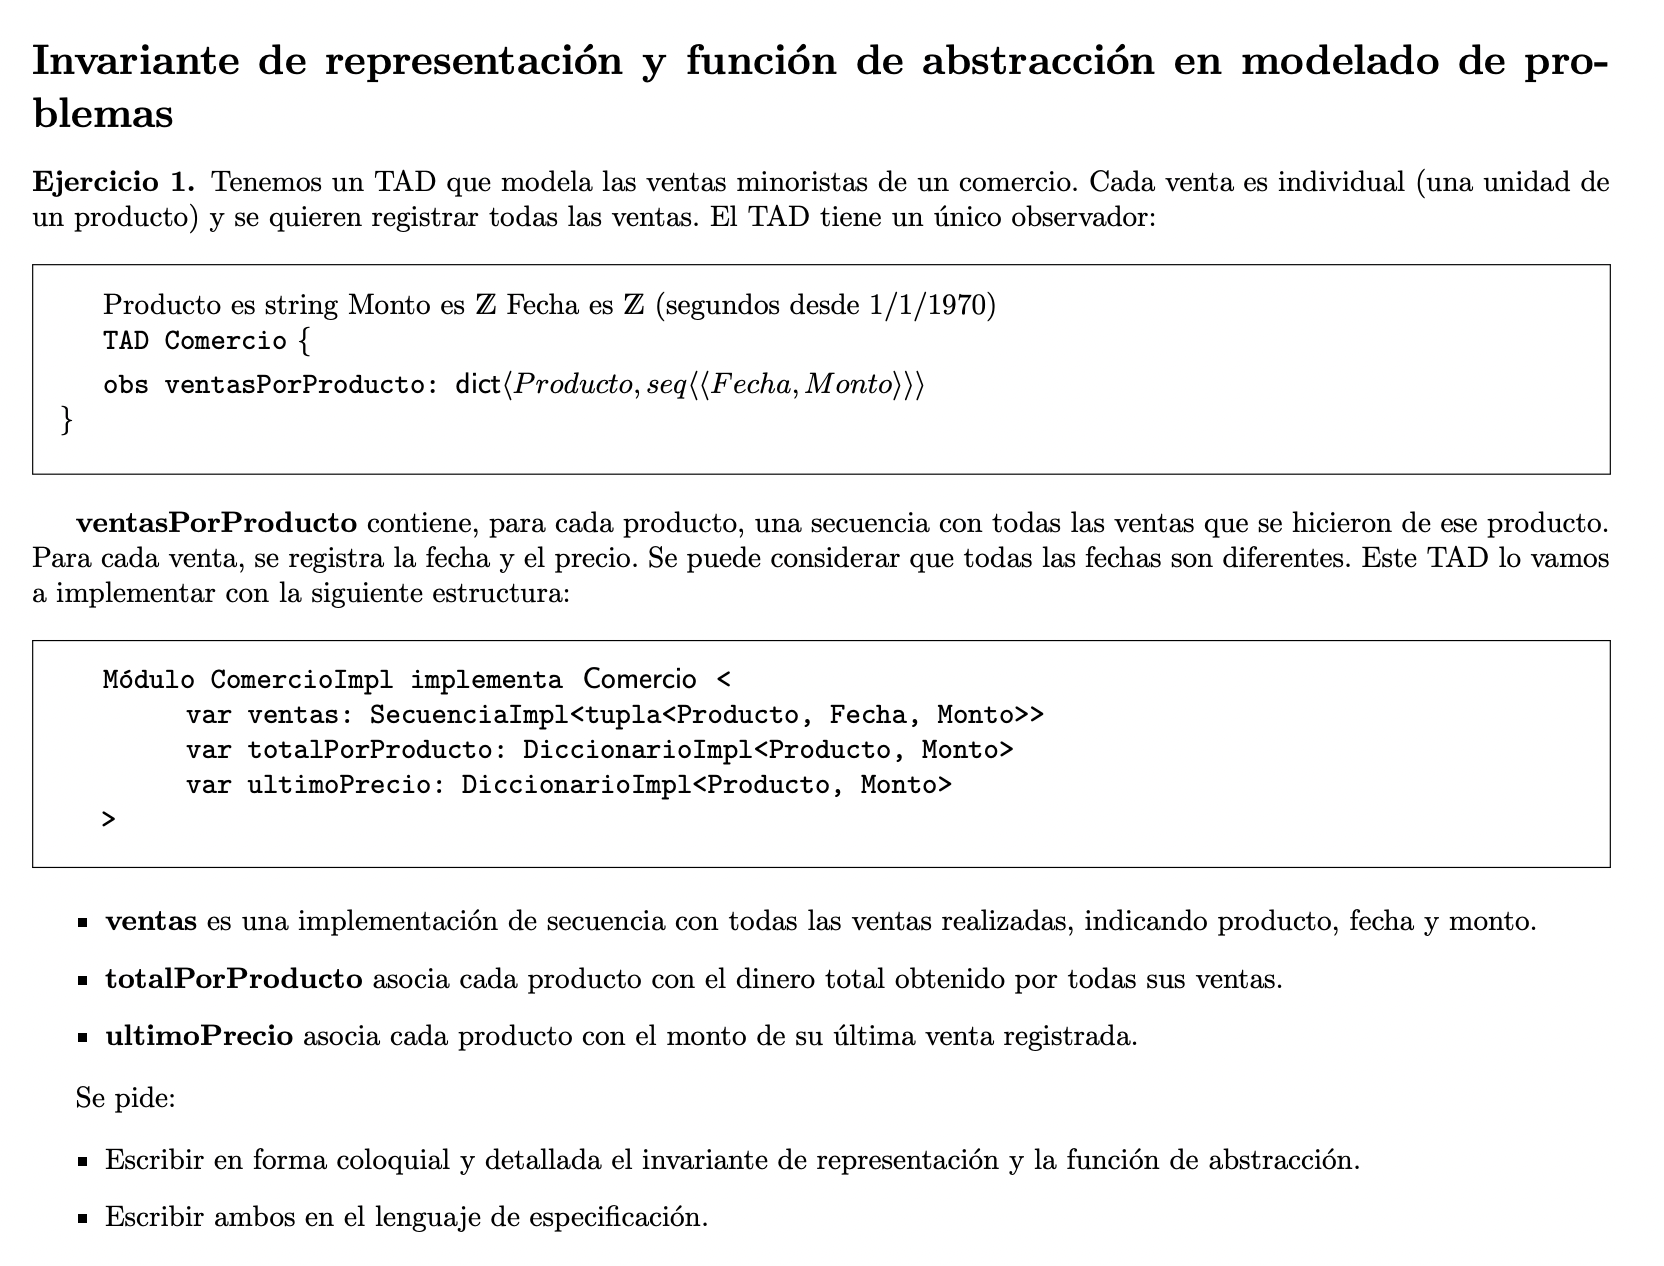
\includegraphics[width=\textwidth]{images/guia_8_ej_1.png}
%   \caption{Enunciado Problema 1}
%   \label{fig:ej_1}
% \end{figure}

% \vspace{1em}
% \Type{Producto}{int}
% \Type{Fecha}{int}
% \Type{Monto}{float}
% \Type{Ventas}{\Clase{SecuenciaImpl}{\Tupla{Producto, Fecha, Monto}}}
% \vspace{1em}
% \begin{ModuloImplements}{ComercioImpl}{Comercio}
%   \begin{Vars}
%     \Var{ventas}{Ventas}
%     \Var{totalPorProducto}{\Clase{DiccionarioImpl}{Producto, Monto}}
%     \Var{ultimoPrecio}{\Clase{DiccionarioImpl}{Producto, Monto}}
%   \end{Vars}

%   \aux{indiceDeFechaMasReciente}{c: ComercioImpl, $i_1$: \ent, $i_2$: \ent}{\ent}{
%     IfThenElse(
%       \\\Indent c.ventas.s[i_1]_1 > c.ventas.s[i_2]_1, i_1, i_2
%     \\\hspace{0.65em})
%   }
%   \aux{indiceUltimoPrecio}{c: ComercioImpl, ventas: Ventas, inicio: \ent}{\ent}{
%     IfThenElse(
%       \\\Indent inicio = |ventas.s| - 1,
%       \\\Indent inicio,
%       \\\Indent indiceDeFechaMasReciente(c, inicio, ultimoPrecio(c, ventas, inicio + 1))
%     \\\hspace{0.65em})
%   }
%   \aux{totalPorProducto}{c: ComercioImpl, producto: Producto}{\ent}{
%     \\\Indent \displaystyle \sum_{i=0}^{|c.ventas.s|-1} IfThenElse(c.ventas.s[i]_0 = producto, c.ventas.s[i]_2, 0)
%   }
%   \vspace{1em}
%   \pred{abs}{ab: \Clase{ArbolBinarioImpl}{T}, ab': \Clase{ArbolBinario}{T}}{
%     Abs
%   }
%   \pred{invRep}{l: \Clase{ListaEnlazada}{T}}{
%     InvRep
%   }
% \end{ModuloImplements}

% \newpage

\SuperTitle{Elección de estructuras}

\Title{Recomendaciones varias para estos ejercicios:}

\par Lo que más conviene es: leer y entender bien el enunciado. Repetir recursivamente hasta entenderlo bien.
\par Siempre, o casi siempre, nos van a dar datos clave en él. Hay que ponerse en el rol de detective. La mayoría de las veces nos vamos
a encontrar con un dato (o más de uno) que está acotado: debemos reconocerlos. Que un dato esté acotado nos va a permitir elegir
casi cualquier casi estructura para representarlo.
\par Los pasos serían:
\\1. Leer bien el enunciado.
\\2. Mirar el apunte de Módulos.
\\3. Ir de los procs de menor complejidad a mayor complejidad.
\\4. Elegir estructuras que nos permitan cumplir las complejidades del \textbf{3} e ir ajustándola para que funcionen con procs de mayor complejidad. 
\par Otra, y última cosa, a veces vamos a tener que elegir si la eficiencia la vamos a tener al escribir o al leer. Pocas veces pasa que la lectura y escritura son eficientes en simultáneo, así que, en muchos ejercicios
nos piden que cumplamos ciertas complejidades para leer (o escribir), pero no para escribir (o leer). Hay veces que sólo nos van a pedir leer, o sólo nos van a pedir escribir. Leamos bien, muy bien, el enunciado. No hace falta pensar la estructura perfecta, solo la mínima posible para que cumpla con lo pedido.

\newpage

\Title{Ejercicio 4}

\begin{figure}[h]
  \centering
  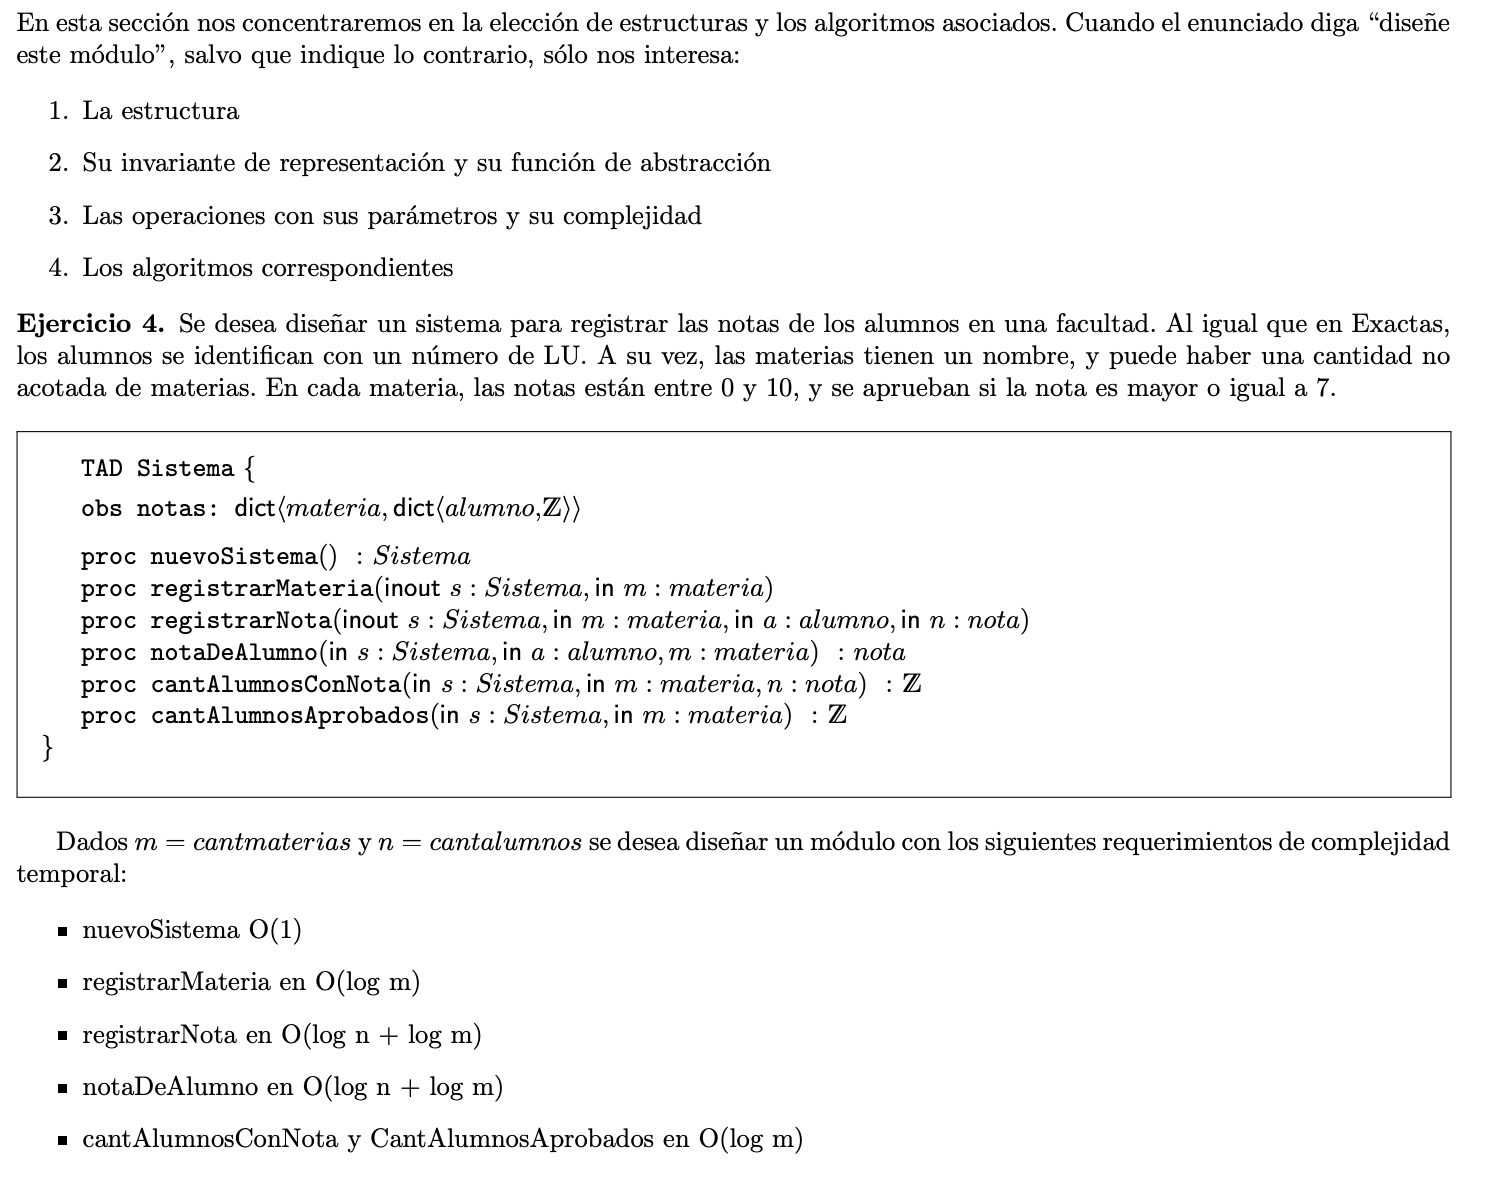
\includegraphics[width=\textwidth]{images/guia_8_ej_4.png}
  \caption{Enunciado Problema 4}
  \label{fig:ej_4}
\end{figure}

Hay dos formas de resolver este ejercicio (posiblemente más). La primera es más intuitiva así que vamos con esa.
Luego de leer bien el enunciado nos damos cuenta de que las \textbf{notas} están acotadas. Solo hay 11 notas posibles, y lo vamos a usar a nuestro favor.


\vspace{1em}
\Type{Alumno}{string}
\Type{Materia}{string}
\Type{Nota}{int}
\vspace{1em}
\begin{ModuloImplements}{SistemaImpl}{Sistema}
  \begin{Vars}
    \Var{notas}{\Clase{DiccionarioLog}{Materia, \Clase{Array}{\Clase{ConjuntoLog}{Alumno}}}}
  \end{Vars}

  \begin{proc}{nuevoSistema}{}{SistemaImpl}
    \begin{ImplementationCode}{470px}
      res.notas:= diccionarioVacío<>() // O(1)

      return res // O(1)
      /**
      * Complejidad final
      * O(1)
      */
    \end{ImplementationCode}
  \end{proc}

  \begin{proc}{registrarMateria}{\Inout s: SistemaImpl, \In m: Materia}{}
    \begin{ImplementationCode}{470px}
      // En algún lado debería haber un requiere que materia aún no está registrada.
      var valor: Array<ConjuntoLog<Alumno>>
          valor:= new Array(11) // O(11) == O(1)
      
      var j: int
          j:= 0
      
      while (j <= 11) do // O(11) == O(1)
        valor[j]:= conjuntoVacío<Alumno>() // O(1)
        j:= j + 1
      endwhile
      
      s.notas.definirRápido(m, valor) // O(log(m))
      /**
       * Complejidad final
       * O(log(m))
       */
    \end{ImplementationCode}
  \end{proc}

  \begin{proc}{registrarNota}{\Inout s: SistemaImpl, \In m: Materia, \In a: Alumno, \In nota: Nota}{}
    \begin{ImplementationCode}{470px}
      // En algún lado debería haber un requiere que ese alumno no tiene una nota registrada.
      // para esa materia. Y que nota está en rango.
      var notasDeMateria: Array<ConjuntoLog<Alumno>>
          notasDeMateria:= s.notas.obtener(m) // O(log(m))
      
      // O(log(n)). Peor caso: Todos los alumnos tienen la misma nota en la misma materia.
      notasDeMateria[nota].agregarRapido(a) // O(log(n))
      notasDeMateria.definir(m, notasDeMateria) // O(log(m))

      /**
       * Complejidad final
       * O(log(m) + log(n))
       */
      \end{ImplementationCode}
  \end{proc}

  \begin{proc}{notaDelAlumno}{\In s: SistemaImpl, \In m: Materia, \In a: Alumno}{Nota}
    \begin{ImplementationCode}{470px}
      // En algún lado debería haber un requiere que ese alumno tiene una nota
      // (convenientemente única) en esa materia.
      var notasDeMateria: Array<ConjuntoLog<Alumno>>
          notasDeMateria:= s.notas.obtener(m) // O(log(m))

      var j: int
      var nota: int
          j:= 0
          nota:= 0

      while (j <= 11) do // O(11 * log(n)) == O(log(n))
        if notasDeMateria[j].pertenece(alumno) then // O(log(n))
          nota:= j
        endif

        j:= j + 1
      endwhile

      return nota
      /**
       * Complejidad final
       * O(log(m) + log(n))
       */
    \end{ImplementationCode}
  \end{proc}

  \begin{proc}{cantAlumnosConNota}{\In s: SistemaImpl, \In m: Materia, \In nota: Nota}{int}
    \begin{ImplementationCode}{470px}
      var notasDeMateria: Array<ConjuntoLog<Alumno>>
          notasDeMateria:= s.notas.obtener(m) // O(log(m))

      return notasDeMateria[nota].tamaño()
      /**
       * Complejidad final
       * O(log(m))
       */
    \end{ImplementationCode}
  \end{proc}

  \begin{proc}{cantAlumnosAprobados}{\In s: SistemaImpl, \In m: Materia}{int}
    \begin{ImplementationCode}{470px}
      var notasDeMateria: Array<ConjuntoLog<Alumno>>
          notasDeMateria:= s.notas.obtener(m) // O(log(m))

      var j: int
      var suma: int
          j:= 7
          suma:= 0

      while (j <= 11) do // O(1) == O(1)
        suma:= suma + cantAlumnosConNota(s, m, j) // O(1)
        j:= j + 1
      endwhile
      /**
       * Complejidad final
       * O(log(m))
       */
    \end{ImplementationCode}
  \end{proc}
\end{ModuloImplements}

\newpage

\Title{Ejercicio 5}

\begin{figure}[h]
  \centering
  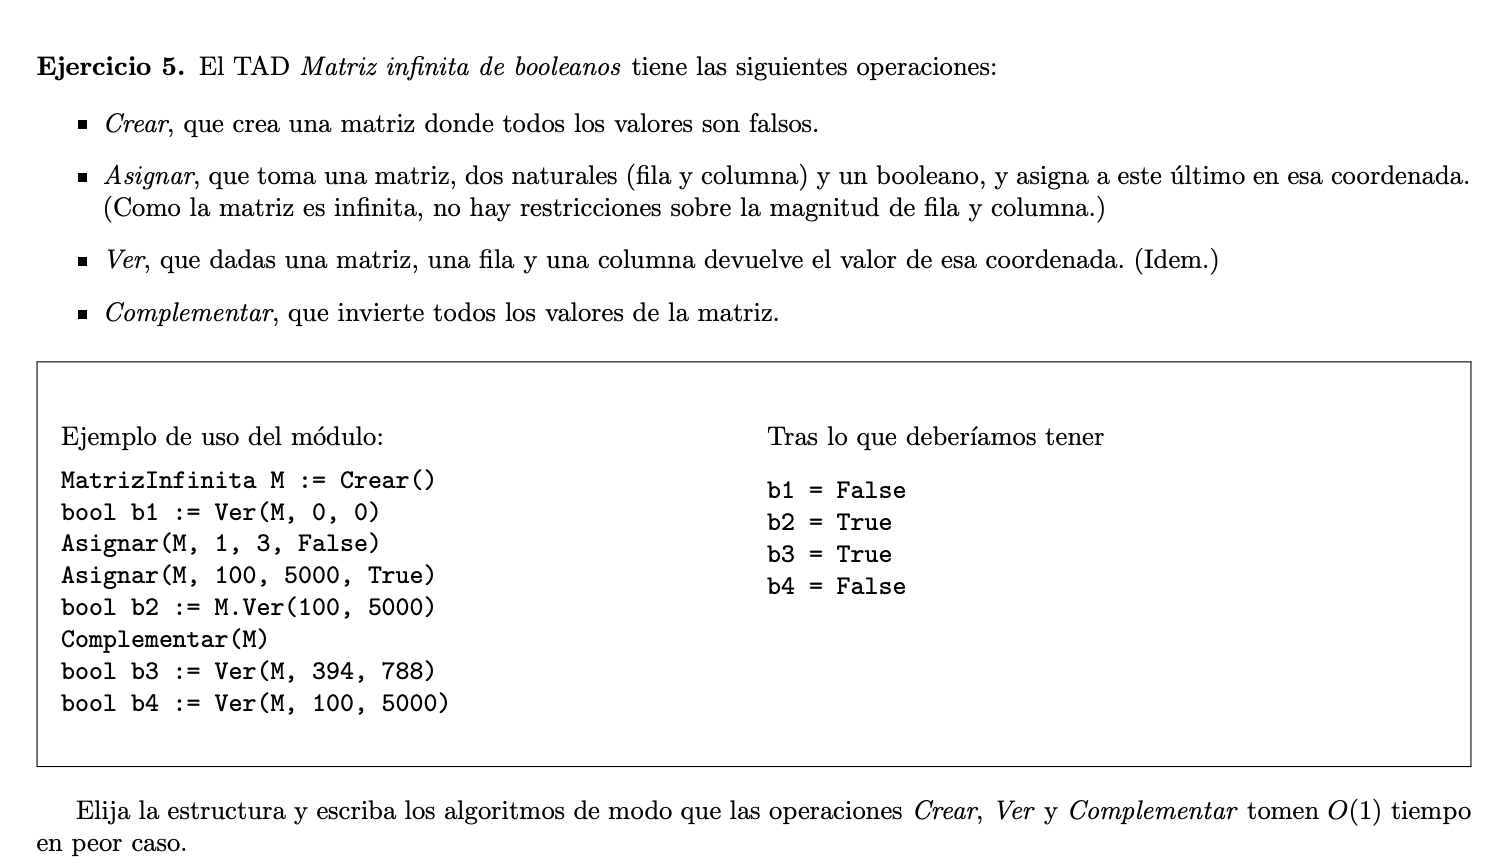
\includegraphics[width=\textwidth]{images/guia_8_ej_5.png}
  \caption{Enunciado Problema 5}
  \label{fig:ej_5}
\end{figure}

\par Nos tenemos que poder dar cuenta después de \textbf{dos} cosas después de nuestro intensivo estudio del enunciado.
\par La primera es que los valores están acotados, solo pueden haber dos casos, true o false. Eso es clave.
\par La segunda es que no nos piden ninguna complejidad para escribir (el ej. busca lectura eficiente), así que: Sacrifiquemos complejidad en ese proc.
\par Con el primer dato, podemos inteligentemente, armar una estructura que nos permita Complementar en O(1).
\par Si recorremos cada uno de los Módulos del apunte, nos vamos a dar cuenta que ninguna estructura nos sirve para leer en O(1), salvo Vector.
\par Así que... tendremos que usar Vector: \textbf{necesitamos} leer un par i,j en O(1).

\vspace{1em}
\Type{Colunna}{int}
\Type{Fila}{int}
\vspace{1em}
\begin{ModuloImplements}{MatrizInfinitaDeBooleanosImpl}{MatrizInfinitaDeBooleanos}
  \begin{Vars}
    \Var{datos}{\Clase{Vector}{\Clase{Vector}{bool}}}
    \Var{estaComplementada}{bool}
  \end{Vars}

  \begin{proc}{agrandarFila}{\Inout m: MatrizInfinitaDeBooleanosImpl, \In f: Fila, \In c: Columna}{}
    \begin{ImplementationCode}{470px}
      if f > m.datos.obtener(f).longitud() then
        int j: int
            j:= 0
        
        while (j <= c) do // O(m)
          // Insertamos false: Valor por default.
          m.datos.obtener(f).agregarAtras(false) // O(f(m)). Amortizado: O(2).
          j:= j + 1 // O(1)
        endwhile
      endif
      /**
       * Complejidad final
       * O(m)
       */
    \end{ImplementationCode}
  \end{proc}

  \begin{proc}{agrandarFilas}{\Inout m: MatrizInfinitaDeBooleanosImpl, \In f: Fila, \In c: Columna}{}
    \begin{ImplementationCode}{470px}
      if f > m.datos.longitud() then
        int j: int
            j:= 0
        
        while (j <= f) do         // O(n * m)
          m.agrandarFila(m, j, c) // O(m)
          j:= j + 1 // O(1)
        endwhile
      endif
      /**
       * Complejidad final
       * O(n * m)
       */
    \end{ImplementationCode}
  \end{proc}

  \comentario{Asignar}

  \begin{proc}{Asignar}{\Inout m: MatrizInfinitaDeBooleanosImpl, \In f: Fila, \In c: Columna, \In v: bool}{}
    \begin{ImplementationCode}{470px}
      m.agrandarVector(m, f, c)                    // O(n * m)
      m.datos.obtener(f).modificarPosicion(c, estaComplementada ? !v : v) // O(1)
      /**
       * Complejidad final
       * O(n * m)
       */
    \end{ImplementationCode}
  \end{proc}

  \comentario{Procs O(1)}

  \begin{proc}{obtenerValor}{\In m: MatrizInfinitaDeBooleanosImpl, \In f: Fila, \In c: Columna}{bool}
    \begin{ImplementationCode}{470px}
      if f >= m.datos.lontitud() || c >= m.datos.obtener(f).longitud() then // O(1)
        // Devolvemos: Valor por default.
        return false // O(1)
      else
        return m.datos.obtener(f).obtener(c) // O(1)
      endif
      /**
       * Complejidad final
       * O(1)
       */
    \end{ImplementationCode}
  \end{proc}

  \begin{proc}{crear}{}{MatrizInfinitaDeBooleanosImpl}
    \begin{ImplementationCode}{470px}
      res.datos:= vectorVacío<>() // O(1)
      res.estaComplementada:= false // O(1)
      return res // O(1)
      /**
       * Complejidad final
       * O(1)
       */
    \end{ImplementationCode}
  \end{proc}

  \begin{proc}{Ver}{\Inout m: MatrizInfinitaDeBooleanosImpl, \In f: Fila, \In c: Columna}{bool}
    \begin{ImplementationCode}{470px}
      var v: bool
          v:= obtenerValor(m, f, c) // O(1)
      
      return estaComplementada ? !v : v // O(1)
      /**
       * Complejidad final
       * O(1)
       */
      \end{ImplementationCode}
  \end{proc}

  \begin{proc}{Complementar}{\Inout m: MatrizInfinitaDeBooleanosImpl}{}
    \begin{ImplementationCode}{470px}
      m.estaComplementada = !m.estaComplementada
      /**
       * Complejidad final
       * O(1)
       */
    \end{ImplementationCode}
  \end{proc}
\end{ModuloImplements}

\newpage


\Title{Ejercicio 6}

\begin{figure}[h]
  \centering
  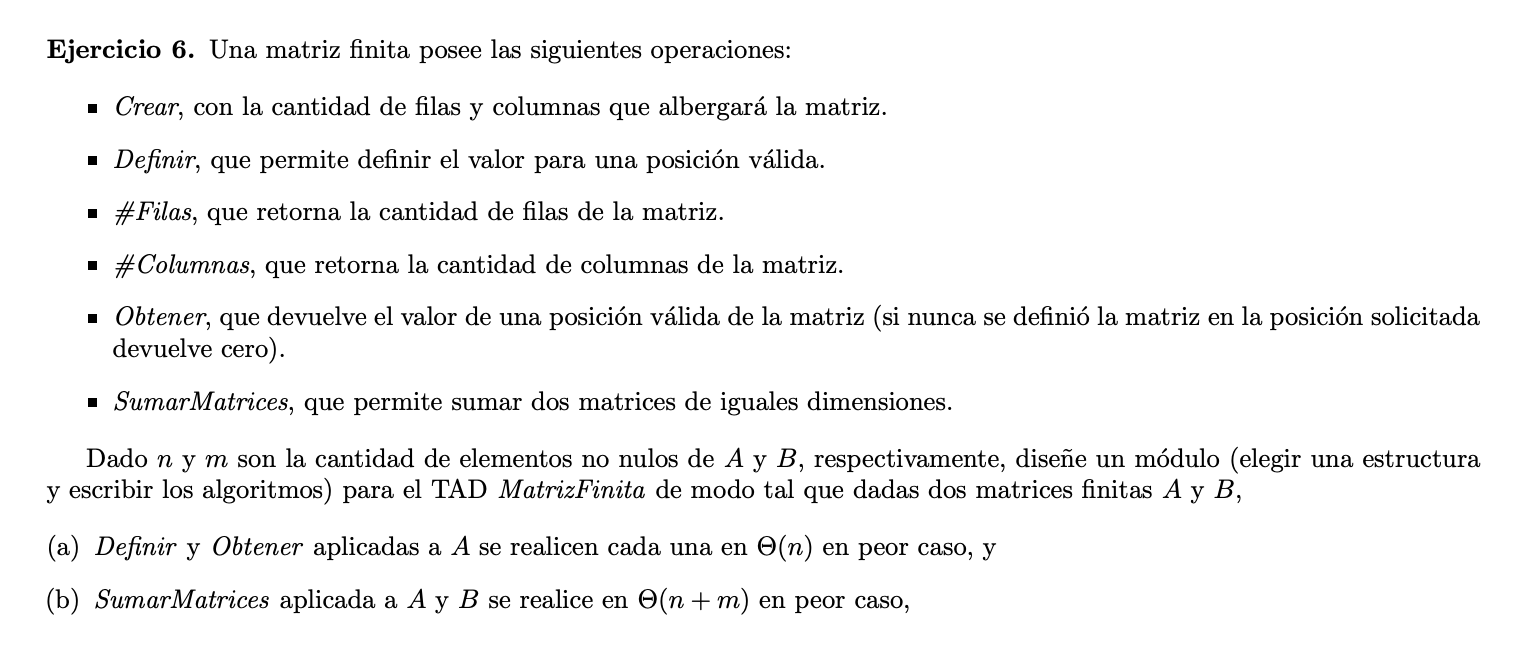
\includegraphics[width=\textwidth]{images/guia_8_ej_6.png}
  \caption{Enunciado Problema 6}
  \label{fig:ej_6}
\end{figure}

\par Nos hablan de \ensuremath{\Theta(n)} en peor caso: Qué sugiere?
% \par Sabemos que la búsqueda lineal es \ensuremath{O(n)}, pero el modelo matemático nos permite tranquilamente decir
% que la búsqueda lineal es \ensuremath{O(n!)}, o \ensuremath{O(n^n)}. Pero la idea es que siempre demos las complejidades
% con la cota más ajustada posible, y dado que la más ajustada posible no siempre es la más exacta, por practicidad se usa O en vez de \ensuremath{\Theta}.
% \par En líneas generales cuando buscamos la complejidad
% no siempre vamos a poder garantizar al 100\% que la cota que proponemos es la más ajustada posible, es por esa razón, que en la práctica no se utiliza \ensuremath{\Theta}.
\par Cuando se habla de \ensuremath{\Theta(n)} en el peor caso, significa que el comportamiento del algoritmo está acotado tanto superior como inferiormente por \ensuremath{n} (Tpeor \ensuremath{\in O(n)} y Tpeor \ensuremath{\in \Omega(n)}).
\par En cambio \ensuremath{O(n)} solo describe una cota superior, lo que permite que el algoritmo sea más eficiente en ciertos casos, incluso 
\ensuremath{O(1)} y aún así cumpliría con \ensuremath{O(n)}.
\par Dicho esto: ¿Por qué nos piden \ensuremath{\Theta} y no \ensuremath{O}? ¿Cambia en algo?
\par Como se mencionó, si nos pidieran que el peor caso es \ensuremath{O(n)}, tranquilamente podríamos diseñar un algoritmo que sea \ensuremath{O(1)} y estaríamos cumpliendo con lo pedido. Pero con \ensuremath{\Theta(n)} no podemos hacer eso.
\par Podríamos usar un Vector de que almacene cosas de tipo Dato (que contenga fila, columna, dato), forzar una búsqueda lineal y siempre mantenernos
en \ensuremath{\Theta(n)}. Esto funcionaría realmente bien para \textbf{Definir} y \textbf{Obtener}.
\par Pero, hay un gran problema... la suma de matrices. Nunca, pero nunca (con las estructuras que podemos usar), vamos a poder cumplir con la complejidad \ensuremath{\Theta(n + m)}, siempre nos vamos a "pasar", ya que, para cada elemento de la matriz B tendremos que buscar en A (Búsqueda Lineal) si existe un \textbf{Dato} con ese par i,j para realizar la suma y eso nos aumentaría la complejidad a \ensuremath{\Theta(n * m)}.
\par Pero, ¿Qué pasa si mantenemos ordenado el Vector? ¿Cuál es el costo de mantener ordenado un Vector a medida que vamos insertando?
\par Podemos hacer una búsqueda lineal, encontrar la posición ideal, y luego: mover a la derecha todos los elementos del vector a partir de esa posición (Búsqueda Binaria también estaría OK) con un costo total de \ensuremath{\Theta(n)}.
\par Mantenerlo ordenado nos a permitir cumplir con la complejidad de la suma de matrices, puesto que, al estar ordenada, por medio de dos punteros podremos recorrer los Vectores de A y B de manera lineal y exacta: \ensuremath{\Theta(n + m)}

\vspace{1em}
\Type{Dato}{\StructField{f}{int}, \Struct{\StructField{c}{int}, \StructField{valor}{int}}}
\Type{Colunna}{int}
\Type{Fila}{int}
\vspace{1em}
\begin{ModuloImplements}{MatrizFinitaImpl}{MatrizFinita}
  \begin{Vars}
    \Var{datos}{\Clase{Vector}{Dato}}
    \Var{nroFilas}{int}
    \Var{nroColumnas}{int}
  \end{Vars}

  \begin{proc}{esMasPrioritario}{\In d1: Dato, \In d2: Dato}{bool}
    \begin{ImplementationCode}{460px}
      return d1.f < d2.f || (d1.f == d2.f && d1.c < d2.c)
    \end{ImplementationCode}
  \end{proc}

  \begin{proc}{actualizarNumeros}{\Inout m: MatrizFinitaImpl, d: Dato}{bool}
    \begin{ImplementationCode}{460px}
      m.nroFilas = m.nroFilas <= d.f ? m.nroFilas : d.f
      m.nroColumnas = m.nroColumnas <= d.c ? m.nroColumnas : d.c
    \end{ImplementationCode}
  \end{proc}

  \begin{proc}{insertarEnOrden}{\Inout m: MatrizFinitaImpl, \In f: Fila, \In c: Columna, \In valor: int}{MatrizFinitaImpl}
    \begin{ImplementationCode}{460px}
      var nuevoDato: Dato
          nuevoDato:= new Dato(f=f, c=c, valor=valor) // Theta(1)

      var j: int                     // Theta(1)
          j:= m.datos.longitud() - 1 // Theta(1)

      while (j > 0 && m.esMasPrioritario(m.datos.obtener(j), nuevoDato)) do // Peor caso: Theta(n)
        m.datos.modificarPosicion(j, m.datos.obtener(j))                    // Theta(1)
        j:= j - 1                                                           // Theta(1)
      endwhile

      if j == -1 then
        m.datos.agregarAtras(nuevoDato)                    // Theta(n)
        m.actualizarNumeros(m, nuevoDato)
        // Peor caso: O(n) dónde n es la cota mas ajustada -> Theta(n).
      else
        m.datos.modificarPosicion(j, nuevoDato) // Theta(1)
      endif
      /**
       * Complejidad final
       * Peor caso: Theta(n)
       */
    \end{ImplementationCode}
  \end{proc}

  \begin{proc}{Crear}{\In f: Fila, \In c: Columna}{MatrizFinitaImpl}
    \begin{ImplementationCode}{470px}
      res.datos:= vectorVacío<>(0)
      res.nroFilas:= 0
      res.nroColumnas:= 0
      return res
      /**
       * Complejidad final
       * O(f * c)
       */
    \end{ImplementationCode}
  \end{proc}

  \begin{proc}{$\#$Filas}{\In m: MatrizFinitaImpl, \In f: Fila, \In c: Columna}{bool}
    \begin{ImplementationCode}{470px}
      return m.nroFilas
      /**
       * Complejidad final
       * O(1)
       */
    \end{ImplementationCode}
  \end{proc}

  \begin{proc}{$\#$Columna}{\In m: MatrizFinitaImpl, \In f: Fila, \In c: Columna}{bool}
    \begin{ImplementationCode}{470px}
      return m.nroColumnas
      /**
       * Complejidad final
       * O(1)
       */
    \end{ImplementationCode}
  \end{proc}

  \begin{proc}{Definir}{\Inout m: MatrizFinitaImpl, \In f: Fila, \In c: Columna, \In v: bool}{}
    \begin{ImplementationCode}{470px}
      m.insertarEnOrden(m, f, c, v)
      /**
       * Complejidad final
       * Theta(n)
       */
    \end{ImplementationCode}
  \end{proc}

  \begin{proc}{Obtener}{\Inout m: MatrizFinitaImpl, \In f: Fila, \In c: Columna}{int}
    \begin{ImplementationCode}{470px}
      var v: int
      var j: int
          j:= 0

      while (j < m.datos.longitud()) do // Búsqueda Lineal en peor caso:  Theta(n)
        if m.datos.obtener(j).f == f && m.datos.obtener(j).c == c then // Theta(1)
          return m.datos.obtener(j).valor                              // Theta(1)
        endif

        j:= j + 1
      endwhile
      
      // Devolver valro default: 0.
      return 0 // Theta(1)
      /**
       * Complejidad final
       * Theta(n)
       */
      \end{ImplementationCode}
  \end{proc}
  \newpage
  \comentario{No estoy del todo de acuerdo de acceder directamente al attr interno "datos" de m2}
  \comentario{Pero no hay un TAD definido  MatrizFinita donde se pueda acceder a un elemento}
  \comentario{por un índice determinado (j1).}
  \comentario{Lo mas coherente sería que el TAD MatrizFinita esté bien definido y que se pueda}
  \comentario{obtener un Dato de una determinada posición.}
  \begin{proc}{SumarMatrices}{\Inout m1: MatrizFinitaImpl, \In m2: MatrizFinitaImpl}{}
    \begin{ImplementationCode}{470px}
      var datosNuevos: Vector<Dato>
      var j1: int
      var j2: int
          datosNuevos:= vectorVacío<>()       // Theta(1)
          j1:= 0                              // Theta(1)
          j2:= 0                              // Theta(1)
      
      while (j1 < m1.datos.longitud() && j2 < m2.datos.longitud()) do // Theta(min(m, n))
        if m1.esMasPrioritario(m1.datos.obtener(j1), m2.datos.obtener(j2)) then
          datosNuevos.agregarAtras(m1.datos.obtener(j1))
          j1:= j1 + 1
        else
          datosNuevos.agregarAtras(m2.datos.obtener(j2))
          j2:= j2 + 1
        endif
      endwhile

      while (j1 < m1.datos.longitud()) do                   // Theta(n)
        datosNuevos.agregarAtras(m1.datos.obtener(j1))      // Theta(n)
        j1:= j1 + 1
      endwhile

      while (j2 < m2.datos.longitud()) do                   // Theta(m)
        datosNuevos.agregarAtras(m2.datos.obtener(j2))      // Theta(m)
        j2:= j2 + 1
      endwhile

      m1.datos = datosNuevos

      var j: int
          j:= 0

      while (j < datosNuevos.longitud()) do            // Theta(n + m)
        actualizarNumeros(m1, datosNuevos.obtener(j)) // Theta(1)
      endwhile
      /**
       * Complejidad final
       * Theta(n + m)
       */
    \end{ImplementationCode}
  \end{proc}
\end{ModuloImplements}



\end{document}